\chapter{Bài 4. Chuyển động thẳng}
\begin{center}
	\textit{(6 tiết)}
\end{center}
\section{MỤC TIÊU DẠY HỌC}
\begin{center}
	\begin{longtable}{|M{2.5cm}|L{12.5cm}|M{2cm}|}
		\hline
		\thead{Biểu hiện\\ năng lực} & \thead{Mục tiêu} & \thead{STT}\\
		\hline
		\multicolumn{3}{|c|}{\textbf{ Năng lực vật lí}}\\
		
		\hline
		1.1& Từ hình ảnh hoặc ví dụ thực tiễn, định nghĩa được độ dịch chuyển. & 1\\
		\hline
		1.3 & So sánh được quãng đường đi được và độ dịch chuyển. &2\\
		\hline
		1.2 & Lập luận để rút ra được công thức tính tốc độ trung bình, định nghĩa được tốc độ theo một phương. & 3\\
		\hline
		1.4 & Dựa vào định nghĩa tốc độ theo một phương và độ dịch chuyển, rút ra được công thức tính và định nghĩa được vận tốc. & 4\\
		\hline
		1.2 &  Dựa trên số liệu cho trước, vẽ được đồ thị độ dịch chuyển – thời gian trong chuyển động thẳng.& 5\\
		\hline
		1.2 & Tính được tốc độ từ độ dốc của đồ thị độ dịch chuyển – thời gian. & 6\\
		\hline
		\hline
		1.2 & Vận dụng được công thức tính tốc độ, vận tốc. & 7\\
		\hline
		\multicolumn{3}{|c|}{\textbf{Năng lực chung}}\\
		\hline
		TC - TH& Tích cực thực hiện các nhiệm vụ GV đặt ra cho các nhóm, tích cực suy luận để đưa ra câu trả lời trong quá trình GV định hướng nội dung học tập	&8 \\
		\hline
		GT - HT & Tích cực đóng góp ý kiến trong quá trình thảo luận, biết sử dụng ngôn ngữ kết hợp với các loại phương tiện phi ngôn ngữ đa dạng để trình bày các kết quả thảo luận nhóm & 10\\
		\hline
	\end{longtable}
\end{center}
\section{THIẾT BỊ DẠY HỌC VÀ HỌC LIỆU}
\begin{itemize}
	\item Tivi/máy chiếu;
	\item SGK;
	\item Phiếu học tập.
\end{itemize}
\section{TIẾN TRÌNH DẠY HỌC}
\subsection{TIẾN TRÌNH}\newpage
\begin{center}
	\begin{longtable}{|L{2.75cm}|C{1.25cm}|L{5cm}|L{3.5cm}|L{4cm}|}
		\hline
		\thead{Tiến trình} & \thead{Mục\\tiêu} & \thead{Nội dung dạy học \\trọng tâm} & \thead{PP,\\ KTDH} & \thead{Phương pháp \\đánh giá}\\
		\hline
	\textbf{Hoạt động 1:} Phân biệt khái niệm quãng đường và độ dịch chuyển	&1, 2  & Phân biệt khái niệm quãng đường và độ dịch chuyển  & PPDH: Đàm thoại& GV đánh giá dựa trên câu trả lời của HS.\newline
	PP đánh giá: quan sát, nghe. \\
		\hline
		\textbf{Hoạt động 2:} Tìm hiểu khái niệm tốc độ	& 3  & Khái niệm và công thức tính tốc độ trung bình, tốc độ tức thời  & PPDH:  Đàm thoại\newline KTDH: Động não& GV đánh giá dựa trên câu trả lời của HS.\newline
		PP đánh giá: quan sát, nghe. \\
		\hline
		\textbf{Hoạt động 3:} Tìm hiểu khái niệm vận tốc	& 4  & Khái niệm và công thức tính vận tốc trung bình, vận tốc tức thời  & PPDH:  Đàm thoại\newline KTDH: Động não& GV đánh giá dựa trên câu trả lời của HS.\newline
		PP đánh giá: quan sát, nghe. \\
		\hline
		\textbf{Hoạt động 4:} Tìm hiểu đồ thị độ dịch chuyển - thời gian	& 5, 6, 8, 10  & Vẽ đồ thị độ dịch chuyển - thời gian từ số liệu cho trước, cách xác định tốc độ tức thời từ đồ thị độ dịch chuyển - thời gian  & PPDH:  Dạy học hợp tác& GV đánh giá dựa trên câu trả lời của HS và kết quả thảo luận nhóm.\newline
		PP đánh giá: quan sát, nghe. \\
		\hline
		\textbf{Hoạt động 5:} Luyện tập	& 6, 7  & Luyện tập tính tốc độ trung bình, vận tốc trung bình trong chuyển động thẳng, từ số liệu cho trước vẽ được đồ thị độ dịch chuyển - thời gian, tính tốc độ tức thời và vận tốc tức thời từ đồ thị độ dịch chuyển - thời gian. & PPDH:  Đàm thoại& GV đánh giá dựa trên bài tập cá nhân của học sinh.\newline
		PP đánh giá: quan sát, nghe. \\
		\hline
	\end{longtable}
\end{center}
\subsection{CÁC HOẠT ĐỘNG HỌC}
% ==========================================================================================
\hoatdong
{
	Tìm hiểu đồ thị độ dịch chuyển - thời gian
}
{\begin{itemize}
		\item HS định nghĩa được độ dịch chuyển.
		\item  HS so sánh được quãng đường đi được và độ dịch chuyển.
	\end{itemize}
	
}
{
	Kết quả trả lời của HS cho các câu hỏi gợi mở của GV:\\
	\textbf{Câu trả lời dự kiến:} 
	\begin{itemize}
		\item Trường hợp nhân vật đi từ O đến B:
		\begin{itemize}
			\item quãng đường đi là $s=OB$;
			\item độ dịch chuyển là $d=OB$.
		\end{itemize}
		\item Trường hợp nhân vật đi từ O đến B rồi về A:
		\begin{itemize}
			\item quãng đường đi là $s=OB+AB$;
			\item độ dịch chuyển là $d=OA$.
		\end{itemize}
	\end{itemize}
}
{\textit{\underline{* GV chuyển giao nhiệm vụ học tập}}\\
	GV giới thiệu cho học sinh về khái niệm quãng đường và độ dịch chuyển.\\
	GV yêu cầu HS xác định độ dịch chuyển và quãng đường đi được của nhân vật trong ví dụ hình bên trong các trường hợp
	\begin{center}
		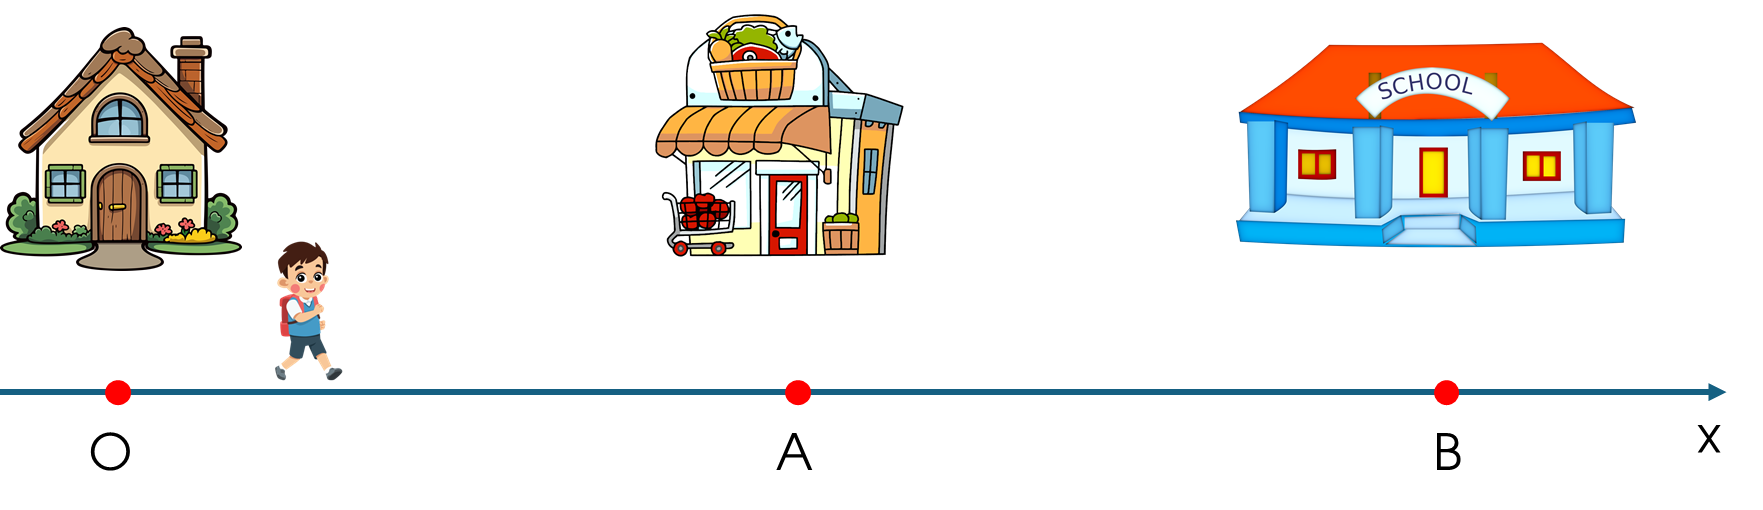
\includegraphics[width=0.9\linewidth]{figs/BAI4-1}
	\end{center}
	\begin{itemize}
		\item nhân vật đi từ nhà đến trường.
		\item nhân vật đi từ nhà đến trường rồi đến cửa hàng tạp hóa.
	\end{itemize}
	\textit{\underline{* HS thực hiện nhiệm vụ học tập}}\\
	HS tích cực trả lời câu hỏi gợi mở của GV.\\
	HS chú ý theo dõi, đặt câu hỏi.
}
% ==========================================================================================
\hoatdong
{
	Tìm hiểu khái niệm tốc độ
}
{\begin{itemize}
		\item HS nêu được tốc độ là đại lượng đặc trưng cho tính chất nhanh, chậm của chuyển động.
		\item HS lập luận rút ra được công thức tính tốc độ trung bình.
	\end{itemize}
	
}
{
	Kết quả trả lời của HS cho các câu hỏi gợi mở của GV:\\
	\textbf{Câu trả lời dự kiến:} Trung bình 1 giây vận động viên bơi được $\SI{2}{\meter}$ ở lần đầu và $\SI{1.79}{\meter}$ ở lần sau. Như vậy, lần đầu vận động viên này bơi nhanh hơn.
}
{\textit{\underline{* GV chuyển giao nhiệm vụ học tập}}\\
GV đặt ra tình huống để HS thảo luận theo nhóm đôi:\\
\textit{Một vận động viên bơi lội người Mỹ đã từng lập kỉ lục thế giới ở nội dung bơi bướm $\SI{100}{\meter}$ và $\SI{200}{\meter}$ với thời gian lần lượt là $\SI{49.82}{\second}$ và $\SI{111.51}{\second}$. Hãy lập luận để xác định vận động viên này bơi nhanh hơn trong trường hợp nào?}\\
Từ câu trả lời của HS, GV dẫn dắt đến khái niệm tốc độ trung bình.\\
GV giới thiệu cho HS khái niệm tốc độ tức thời.\\
GV đặt câu hỏi: \textit{Vậy số chỉ trên tốc kế là tốc độ trung bình hay tốc độ tức thời?}\\
\textit{\underline{* HS thực hiện nhiệm vụ học tập}}\\
HS tích cực trả lời câu hỏi gợi mở của GV.\\
HS chú ý theo dõi, đặt câu hỏi.\\
\textit{\underline{* HS báo cáo kết quả thực hiện nhiệm vụ học tập}}\\
GV lần lượt mời 1 HS trả lời câu hỏi và 1 HS khác nhận xét câu trả lời.\\
HS theo dõi, nhận xét, đặt câu hỏi.\\
GV chỉnh lí, hợp thức hoá kiến thức.
}
% ==========================================================================================
\hoatdong
{
	Tìm hiểu khái niệm vận tốc
}
{\begin{itemize}
		\item HS dựa vào định nghĩa tốc độ theo một phương và độ dịch chuyển, rút ra được công thức tính và định nghĩa được vận tốc.
		\item HS phân biệt được tốc độ trung bình và vận tốc trung bình.
	\end{itemize}

}
{
	Câu trả lời của HS cho câu hỏi gợi mở do GV đưa ra:\\
	\textbf{Câu trả lời dự kiến:} Cần phải biết thêm hướng chuyển động của hai người mới có thể xác định được vị trí gặp nhau.
}
{\textit{\underline{* GV chuyển giao nhiệm vụ học tập}}\\
	GV đặt câu hỏi gợi mở: \textit{Có hai người đi xe máy khởi hành cùng lúc từ thành phố A và thành phố B cách nhau $\SI{40}{\kilo\meter}$ với tốc độ không đổi $\SI{40}{\kilo\meter/\hour}$ và $\SI{60}{\kilo\meter/\hour}$ trên một đường thẳng. Em có thể xác định được thời điểm hai người gặp nhau không? Vì sao?}\\
	Từ câu trả lời của HS, GV rút ra kết luận: \textit{Tốc độ không cho biết hướng chuyển động. Trong các bài toán khảo sát vị trí của vật, ta cần quan tâm đến độ dịch chuyển của vật theo thời gian. Thay đại lượng $s$ trong công thức tốc độ trung bình bằng độ dịch chuyển $\vec{d}$ ta có được đại lượng mới, được gọi là vận tốc trung bình $\vec{v}_{\text{tb}}=\dfrac{\vec{d}}{\Delta t}=\dfrac{\Delta \vec{x}}{\Delta t}$.}\\
	GV đặt câu hỏi để đi đến phần lưu ý: \textit{Vậy khi nào thì tốc độ trung bình bằng với độ lớn của vận tốc trung bình?}\\
	GV giới thiệu khái niệm vận tốc tức thời.\\
	\textit{\underline{* HS thực hiện nhiệm vụ học tập}}\\
	HS tích cực trả lời câu hỏi gợi mở của GV.\\
	HS chú ý theo dõi, đặt câu hỏi.\\
	\textit{\underline{* HS báo cáo kết quả thực hiện nhiệm vụ học tập}}\\
	GV lần lượt mời 1 HS trả lời câu hỏi và 1 HS khác nhận xét câu trả lời.\\
	HS theo dõi, nhận xét, đặt câu hỏi.\\
	GV chỉnh lí, hợp thức hoá kiến thức.
}
% ==========================================================================================
\hoatdong
{
	Tìm hiểu đồ thị độ dịch chuyển - thời gian
}
{\begin{itemize}
		\item HS vẽ được đồ thị độ dịch chuyển - thời gian từ số liệu cho trước.
		\item HS xác định được tốc độ tức thời, vận tốc tức thời từ đồ thị độ dịch chuyển - thời gian.
	\end{itemize}
	
}
{
	Kết quả thảo luận nhóm của HS.
}
{\textit{\underline{* GV chuyển giao nhiệm vụ học tập}}\\
	GV ôn tập lại cho HS phần đồ thị hàm số bậc nhất, nội dung ôn tập như sau:\\
	Đồ thị hàm số $y=ax+b\ \left(a\neq0\right)$ là đường thẳng.
	\begin{center}
		\begin{tabular}{M{8cm}M{8cm}}
			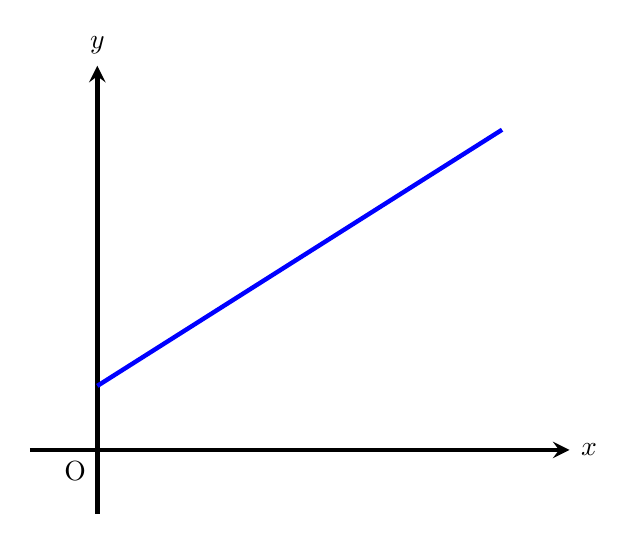
\begin{tikzpicture}  
				\begin{axis}[  ultra thick,
					xmin=-1,  
					xmax=7,  
					ymin=-1,  
					ymax=6, 
					samples=300,
				xtick=\empty,
				ytick=\empty,
					yticklabels=\empty,
					xticklabels=\empty,
					axis lines=center, 
					xlabel=$x$, 		ylabel=$y$,
					every axis y label/.style={at=(current axis.above origin),anchor=south},  
					every axis x label/.style={at=(current axis.right of origin),anchor=west},  ]
					\addplot [ultra thick, blue, smooth, domain=0:6] {1+2*x/3};
					\node[below left] at (axis cs: 0, 0) {O}; 
				\end{axis}  
			\end{tikzpicture} &
			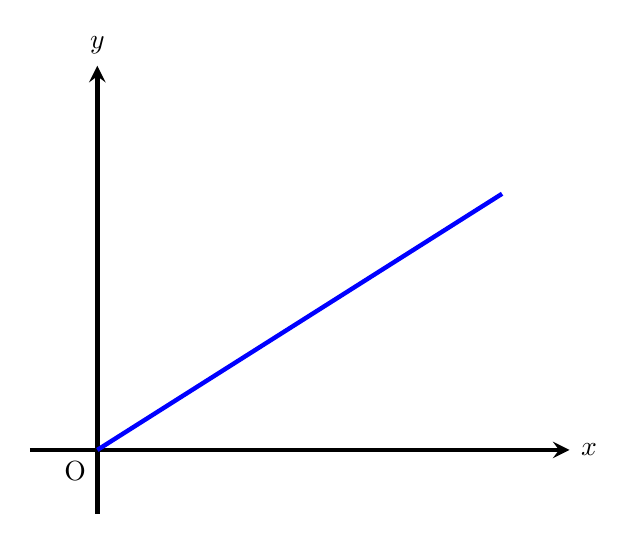
\begin{tikzpicture}  
				\begin{axis}[  ultra thick,
					xmin=-1,  
					xmax=7,  
					ymin=-1,  
					ymax=6, 
					xtick=\empty,
					ytick=\empty,
					samples=300,
					yticklabels=\empty,
					xticklabels=\empty,
					axis lines=center, 
					xlabel=$x$, 		ylabel=$y$,
					every axis y label/.style={at=(current axis.above origin),anchor=south},  
					every axis x label/.style={at=(current axis.right of origin),anchor=west},  ]
					\addplot [ultra thick, blue, smooth, domain=0:6] {2*x/3}; 
					\node[below left] at (axis cs: 0, 0) {O};
				\end{axis}  
			\end{tikzpicture}\\
			$b\neq 0$ & $b=0$
		\end{tabular}
	\end{center}
	\begin{center}
		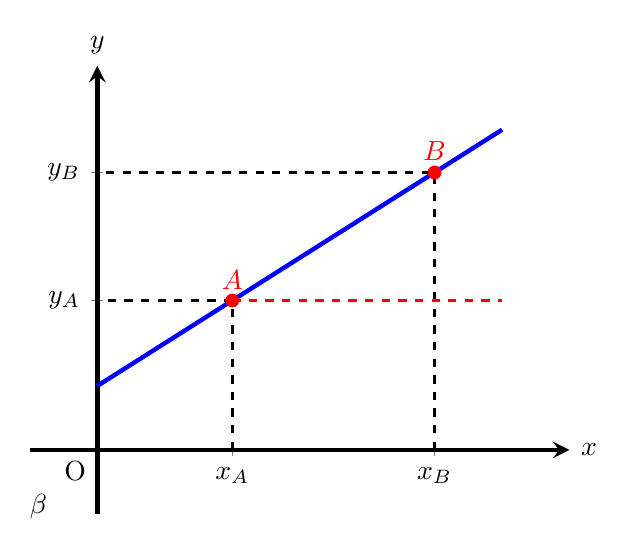
\begin{tikzpicture}  
			\begin{axis}[  ultra thick,
				xmin=-1,  
				xmax=7,  
				ymin=-1,  
				ymax=6, 
				samples=300,
				xtick={2, 5},
				ytick={2.3333, 4.3333},
				yticklabels={$y_A$, $y_B$},
				xticklabels={$x_A$, $x_B$},
				axis lines=center, 
				xlabel=$x$, 		ylabel=$y$,
				every axis y label/.style={at=(current axis.above origin),anchor=south},  
				every axis x label/.style={at=(current axis.right of origin),anchor=west},  ]
				\coordinate (A) at (axis cs: 2, 2.3333);
				\coordinate (B) at (axis cs: 5, 4.3333);
				\coordinate (C) at (axis cs: 6, 2.3333);
				\addplot [ultra thick, blue, smooth, domain=0:6] {1+2*x/3};
				\node[below left] at (axis cs: 0, 0) {O}; 
				\draw[dashed, line width=1pt] (axis cs: 2,0)--(A)--(axis cs:0,2.3333);
				\draw[dashed, line width=1pt] (axis cs: 5,0)--(B)--(axis cs:0,4.3333);
				\draw[dashed, line width=1pt, red] (A)--(axis cs:6,2.3333);
				\fill[red]   (A) circle[radius=2.5pt]  node [above] {$A$};
				\fill[red]   (B) circle[radius=2.5pt]  node [above] {$B$};
			\end{axis} 
			\tkzMarkAngle[size=0.75cm,color=red, line width=1pt](C,A,B);
			\tkzLabelAngle[color=black,pos=1.2](C,A,B){$\beta$}; 
		\end{tikzpicture}
		
	\end{center}
}

